\subsection{The Factor-Tree Planner}
\label{sec:tensors:preprocessing}
Approaches to tensor-network contraction that do not modify the input tensor network (e.g., \textbf{LG}) are inherently limited by the ranks of the input tensors. If a tensor network has a rank $r$ tensor, then all contraction trees have max rank of at least $r$. This is a problem for tensor networks with high-rank tensors. 

One example of tensor networks that may contain high-rank tensors are the networks obtained by the reduction from model counting. The tensor network produced from a formula $\varphi$ contains a tensor representing each variable $x$, where the rank of this tensor is the number of appearances of $x$ in $\varphi$ (e.g., the rank $4$ tensor for $y$ in Figure \ref{fig:wmc-example}). For many benchmarks, where a single variable might appear tens or even hundreds of times, this reduction will therefore produce tensor networks containing tensors of infeasibly-high rank. Reductions exist from model counting on arbitrary formulas to model counting on formulas where the number of appearances of each variables is small. However, existing reductions do not consider the carving width of the resulting incidence graph and so often do not significantly improve the max rank of available contraction trees. 

We introduce here a novel planning method \textbf{Factor-Tree} that avoids this barrier by preprocessing the input tensor network. Our insight is that a tree decomposition for the incidence graph of $\varphi$ can be used as a guide to introduce new variables in a principled way, so that the resulting tensor network has good contraction trees. In the language of tensors, introducing new variables corresponds to \emph{factoring}: replacing each high-rank tensor $A$ with a tensor network $N_A$ of low-rank tensors that contracts to $A$. The key idea of \textbf{FT}, then, is to use a tree decomposition for the structure graph to factor high-rank tensors.

We state this new result as Theorem \ref{thm:factorable-tree}. Since not all tensors can be factored in the ways that we require for this theorem and for \textbf{FT}, we first characterize the required property: that every tensor is factorable as an arbitrary tree of tensors:

% In fact, we can generalize this result to a wider class of tensor networks. To use a tree decomposition as a guide to simplify a tensor network we ultimately require that we can identify each tensor with a tensor network whose structure graph (excluding the free vertex) is an arbitrary tree. We call this property \emph{tree factorable}:

% We demonstrate an algorithm to find in polynomial time a tensor network, consisting only of rank 3 tensors, whose contraction is the model count of $F$. Moreover, we prove that the resulting tensor network has a good contraction tree if the guiding tree decomposition has small width.
%Instead of directly proving these claims (which are ultimately a corollary of Theorem \ref{thm:factorable-tree}), we generalize this result to a wider class of tensor networks. 

\begin{definition} \label{def:tree-factorable}
A tensor $A$ is \emph{tree factorable} if, for every tree $T$ whose leaves are $\tdim{A}$ (called a \emph{dimension tree} of $A$), there is a tensor network $N_A$ and a bijection $g_A: \V{T} \rightarrow N_A$ s.t.
\begin{enumerate}
\item $A$ is the contraction of $N_A$,
\item $g_A$ is an isomorphism between $T$ and the structure graph of $N_A$ with the free vertex (and incident edges) removed,
\item for every index $i$ of $A$, $i$ is an index of $g_A(i)$, and
\item for some index $i$ of $A$, the bond dimension of $N_A$ is no bigger than $|\domain{i}|$. % $\max_{i \in \tnbound{N}} |\domain{i}| \leq \max_{i \in \tdim{A}} |\domain{i}|$.
\end{enumerate}
\end{definition}
All tensors in the reduction of Theorem \ref{thm:wmc-reduction} from weighted model counting to tensor networks are tree factorable. A tensor network $N_A$ that satisfies properties 1, 2, and 3 of Definition \ref{def:tree-factorable} for some tree is called a \emph{Hierarchical Tucker representation} of $A$ \cite{Grasedyck10}. Property 4 ensures the result of Theorem \ref{thm:factorable-tree} has small bond dimension.

% In \cite{Grasedyck10}, a tree $T$ as in Definition \ref{def:tree-factorable} is called a \emph{dimension tree} of the tensor $A$, and a tensor network $N$ that satisfies properties 1, 2, and 3 for a given dimension tree of $A$ is called a \emph{Hierarchical Tucker representation} of $A$. For every tensor $A$ and dimension tree, a hierarchical Tucker representation of $A$ trivially exists with bond dimension $|\domain{A}|$, but a representation may not exist with smaller bond dimension. Limiting the bond dimension in property 4 ensures that the tensor networks we produce in Theorem \ref{thm:factorable-tree} also have small bond dimension.

We now state the main result of this section, which allows us to use a tree decomposition for the structure graph of a tensor network (containing only tree factorable tensors) to factor each tensor in the network and find a contraction tree of low max rank for the resulting network:
\begin{figure}[t]
	\centering
	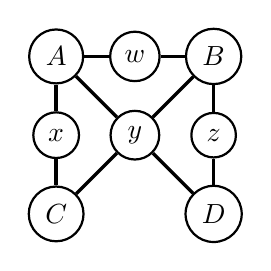
\begin{tikzpicture}
\begin{scope}[every node/.style={circle,thick,draw}]
    \node (C) at (-1,-1) {$C$};
    \node (x) at (-1,0) {$x$};
    \node (A) at (-1,1) {$A$};
    \node (y) at (0,0) {$y$};
    \node (w) at (0,1) {$w$};
    \node (D) at (1,-1) {$D$};
    \node (z) at (1,0) {$z$};
    \node (B) at (1,1) {$B$};
\end{scope}

\begin{scope}[every node/.style={fill=white,circle},
              every edge/.style={draw=black,very thick}]
    \path [-] (A) edge (w);
    \path [-] (A) edge (x);
    \path [-] (A) edge (y);
    \path [-] (B) edge (w);
    \path [-] (B) edge (y);
    \path [-] (B) edge (z);
    \path [-] (C) edge (x);
    \path [-] (C) edge (y);
    \path [-] (D) edge (y);
    \path [-] (D) edge (z);
\end{scope}
\end{tikzpicture}
	\hspace{1cm}
	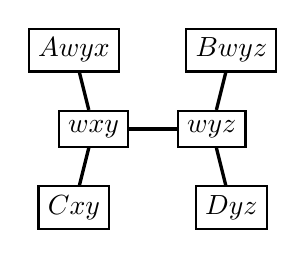
\begin{tikzpicture}
\begin{scope}[every node/.style={rectangle,thick,draw}]
    \node (1) at (-1,1) {$Awyx$};
    \node (2) at (-1,-1) {$Cxy$};
    \node (3) at (-0.75,0) {$wxy$};
    \node (4) at (0.75,0) {$wyz$};
    
    \node (5) at (1,1) {$Bwyz$};
    \node (6) at (1,-1) {$Dyz$};
\end{scope}

\begin{scope}[every node/.style={fill=white,circle},
              every edge/.style={draw=black,very thick}]
    \path [-] (1) edge (3);
    \path [-] (2) edge (3);
    \path [-] (3) edge (4);
    \path [-] (4) edge (5);
    \path [-] (4) edge (6);
\end{scope}
\end{tikzpicture}
	\hspace{1cm}
	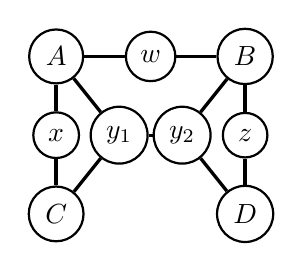
\begin{tikzpicture}
\begin{scope}[every node/.style={circle,thick,draw}]
    \node (C) at (-1.2,-1) {$C$};
    \node (x) at (-1.2,0) {$x$};
    \node (A) at (-1.2,1) {$A$};
    \node (y1) at (-0.4,0) {$y_1$};
    \node (y2) at (0.4,0) {$y_2$};
    \node (w) at (0,1) {$w$};
    \node (D) at (1.2,-1) {$D$};
    \node (z) at (1.2,0) {$z$};
    \node (B) at (1.2,1) {$B$};
\end{scope}

\begin{scope}[every node/.style={fill=white,circle},
              every edge/.style={draw=black,very thick}]
    \path [-] (A) edge (w);
    \path [-] (A) edge (x);
    \path [-] (A) edge (y1);
    \path [-] (B) edge (w);
    \path [-] (B) edge (y2);
    \path [-] (B) edge (z);
    \path [-] (y1) edge (y2);
    \path [-] (C) edge (x);
    \path [-] (C) edge (y1);
    \path [-] (D) edge (y2);
    \path [-] (D) edge (z);
\end{scope}
\end{tikzpicture}
	\caption{\label{fig:factor-example} When FT is run on the shown initial tensor network (left) using the shown tree decomposition (middle), \textbf{FT} produces a factored tensor network (right). Tensors of rank 3 or smaller are unchanged, and the tensor for $y$ is factored into two tensors, $y_1$ and $y_2$, each of rank 3. The factored tensor network has a contraction tree of max rank 3 while the initial tensor network only has contraction trees of max rank 4 or higher.}
\end{figure}

\begin{theorem} \label{thm:factorable-tree}
Let $N$ be a tensor network of tree-factorable tensors s.t. $|\tnfree{N}| \leq 3$ and the structure graph of $N$ has a tree decomposition of width $w \geq 1$.

Then for each $A \in N$ there is a tensor network $N_A$ whose contraction is $A$ that consists only of rank 3 or smaller tensors. Moreover, the disjoint union of these networks, $M = \cup_{A \in N} N_A$, is a tensor network that contracts to $\tntensor{N}$, has the same bond dimension as $N$, and has a contraction tree of max rank no larger than $\ceil{4(w+1)/3}$.
\end{theorem}
\begin{proof}
The proof proceeds in five steps: (1) compute the factored tensor network $M$, (2) construct a graph $H$ that is a simplified version of the structure graph of $M$, (3) construct a carving decomposition $S$ of $H$, (4) bound the width of $S$, and (5) use $S$ to find a contraction tree for $M$. Working with $H$ instead of directly working with the structure graph of $M$ allows us to cleanly handle tensor networks with free indices.

\textbf{Part 1: Factoring the network.}
Let $G$ be the structure graph of $N$ with all degree 0 vertices removed; $G$ must also have a tree decomposition of width $w$. Moreover, the image of $\eincf{G}: \E{G} \rightarrow 2^{\V{G}}$ is an edge clique cover of $G$. Thus using Lemma \ref{lemma:tree-simplification} we can construct a tree decomposition $(T, \chi)$ of $G$ and a bijection $g: \E{G} \rightarrow \Lv{T}$ such that $\chi \circ g = \eincf{G}$ and $width_t(T, \chi) \leq w$.

Next, for each $v \in \V{G}$, define $T_v$ to be the smallest connected component of $T$ containing $\{g(i) ~:~i \in \vinc{H}{v} \}$. Consider each $A \in N$. If $\tnfree{A} = \emptyset$, let $N_A = \{A\}$; thus $\tntensor{N_A} = A$ and the tensor of $N_A$ has rank 0. Otherwise, observe that $T_A$ is a dimension tree of $A$. We can therefore factor $A$ with $T_A$ using Definition \ref{def:tree-factorable} to get a tensor network $N_A$ whose contraction is $A$ and a bijection $g_A: \V{T_A} \rightarrow N_A$. Moreover, every node of $T_A$ has degree 3 or smaller and so, by Definition \ref{def:tree-factorable}, $N_A$ consists only of rank 3 or smaller tensors.

Define $M = \cup_{A \in N} N_A$ and let $G'$ be the structure graph of $M$ with free vertex $\fv'$. The remainder of the proof is devoted to bounding the carving width of $G'$.

\textbf{Part 2: Constructing a simplified structure graph of $M$.} In order to easily characterize $G'$, we define a new, closely-related graph $H$ by taking a copy of $T_v$ for each $v \in \V{G}$ and connecting these copies where indicated by $g$. Formally, the vertices of $H$ are $\{(v, n) : v \in \V{G}, n \in \V{T_v}\}$. For every $v \in \V{G}$ and every arc in $T$ with endpoints $n, m \in \V{T_v}$, we add an edge between $(v, n)$ and $(v, m)$. Moreover, for each $e \in \E{G}$ incident to $v, w \in \V{G}$, we add an edge between $(v, g(e))$ and $(w, g(e))$. 

We will prove in Part 5 that the carving width of $G'$ is bounded from above by the carving width of $H$. We therefore focus in Part 3 and Part 4 on bounding the carving width of $H$. It is helpful for this to define the two projections $\pi_G : \V{H} \rightarrow \V{G}$ and $\pi_T : \V{H} \rightarrow \V{T}$ that indicate respectively the first or second component of a vertex of $H$. 
% For each $v \in \V{G}$, define $H_v = \pi_G^{-1}(v)$. Thus the sets $H_v$ form a partition of $\V{H}$. 

% This ensures that $H \cap H_v$ is isomorphic to $T_v$ and so $H \cap H_v$ is a tree with $|\vinc{G}{v}|$ leaves.

% The map $f: \E{G} \rightarrow \E{H}$ constructed in this way is an injection and satisfies property 3 above. Moreover, since $g(\vinc{G}{v})$ is exactly the leaves of $T_v$, each leaf $\ell \in \Lv{H \cap H_v}$ is incident to exactly one edge in the range of $f$, namely $f(g^{-1}(\ell))$.

\begin{figure}[t]
	\centering
	%\begin{tikzpicture}
\begin{scope}[every node/.style={fill, circle, inner sep=0pt, outer sep=0, minimum size=5pt}]
    \node[label={[xshift=5pt]$n$}] (n) at (0, 0) {};
\end{scope}

\draw[thick] (n) -- (0, 2) node [midway, left] {$a$};
\draw[thick] (n) -- (-1.73, -1) node [midway, above] {$b$};
\draw[thick] (n) -- (1.73, -1) node [midway, above] {$c$};
\end{tikzpicture}
	%\hspace{1cm}
	\begin{tikzpicture}
% Center node
\node[fill, circle, inner sep=0pt, outer sep=0, minimum size=5pt, label={[xshift=8pt, yshift=-5pt]$y_n$}] (yn) at (0, 0) {};

% Minor nodes
\begin{scope}[every node/.style={fill, circle, inner sep=0pt, outer sep=0, minimum size=3pt}]
    \draw[thick] (yn) -- node[pos=0.75, label=right:{$z_{n,a}$}, minimum size=5pt] (zna) {} 
    node[pos=0.525] (Ina1) {} node[pos=0.375] (Ina2) {} node[pos=0.225] (Ina3) {} (0,2);
    \node[left=0.5 of Ina1] (Hna1) {};
    \node[left=0.5 of Ina2] (Hna2) {};
    \node[left=0.5 of Ina3] (Hna3) {};
    
    \draw[thick] (yn) -- node[pos=0.75, label={[xshift=-5pt,yshift=-5pt]$z_{n,b}$}, minimum size=5pt] (znb) {}
    node[pos=0.525] (Inb1) {} node[pos=0.375] (Inb2) {} node[pos=0.225] (Inb3) {} (-1.73, -1);
    \node[below right=0.25 and 0.1 of Inb1] (Hnb1) {};
    \node[below right=0.25 and 0.1 of Inb2] (Hnb2) {};
    \node[below right=0.25 and 0.1 of Inb3] (Hnb3) {};
    
    \draw[thick] (yn) -- node[pos=0.75, label={[xshift=5pt,yshift=-5pt]$z_{n,c}$}, minimum size=5pt] (znc) {}
    node[pos=0.525] (Inc1) {} node[pos=0.375] (Inc2) {} node[pos=0.225] (Inc3) {} (1.73, -1);
    \node[below left=0.25 and 0.1 of Inc1] (Hnc1) {};
    \node[below left=0.25 and 0.1 of Inc2] (Hnc2) {};
    \node[below left=0.25 and 0.1 of Inc3] (Hnc3) {};
    
    % \node[left=5 of zna, label=right:{$z_{\ell,a}$}, minimum size=5pt] (zla) {};
    % \node[left=5 of Ina1] (Ila1) {};
    % \node[left=5 of Ina2] (Ila2) {};
    % \node[left=5 of Ina3] (Ila3) {};
    % \node[left=5 of Hna1] (Hla1) {};
    % \node[left=5 of Hna2] (Hla2) {};
    % \node[left=5 of Hna3] (Hla3) {};
    
    \draw[thick] (-3, 0.52) -- node[pos=0.6825, label=right:{$z_{\ell,a}$}, minimum size=5pt] (zna) {}
    node[pos=0.39] (Ila1) {} node[pos=0.195] (Ila2) {} node[pos=0] (Ila3) {} (-3,2);
    \node[left=0.5 of Ila1] (Hla1) {};
    \node[left=0.5 of Ila2] (Hla2) {};
    \node[left=0.5 of Ila3] (Hla3) {};
\end{scope}

% \node at (zna) [above right] {$y_n$};
%\draw[thick] (yn) -- (0, 2);
%\draw[thick] (yn) -- (-1.73, -1);
%\draw[thick] (yn) -- (1.73, -1);

\draw[thick] (Ina1) -- (Hna1);
\draw[thick] (Ina2) -- (Hna2);
\draw[thick] (Ina3) -- (Hna3);
\draw[decoration={brace,raise=3pt},decorate] (Ina1) -- node[right=4pt] {$I_{n,a}$} (Ina3);
\draw[decoration={brace,mirror,raise=3pt},decorate] (Hna1) -- node[left=4pt] {$H_{n,a}$} (Hna3);

\draw[thick] (Inb1) -- (Hnb1);
\draw[thick] (Inb2) -- (Hnb2);
\draw[thick] (Inb3) -- (Hnb3);
\draw[decoration={brace,raise=3pt},decorate] (Inb1) -- node[above left=1pt and 1pt] {$I_{n,b}$} (Inb3);
\draw[decoration={brace,mirror,raise=3pt},decorate] (Hnb1) -- node[below=6pt] {$H_{n,b}$} (Hnb3);

\draw[thick] (Inc1) -- (Hnc1);
\draw[thick] (Inc2) -- (Hnc2);
\draw[thick] (Inc3) -- (Hnc3);
\draw[decoration={brace,mirror,raise=3pt},decorate] (Inc1) -- node[above right=1pt and 1pt] {$I_{n,c}$} (Inc3);
\draw[decoration={brace,raise=3pt},decorate] (Hnc1) -- node[below=6pt] {$H_{n,c}$} (Hnc3);


\draw[thick] (Ila1) -- (Hla1);
\draw[thick] (Ila2) -- (Hla2);
\draw[thick] (Ila3) -- (Hla3);
\draw[decoration={brace,raise=3pt},decorate] (Ila1) -- node[right=4pt] {$I_{\ell,a}$} (Ila3);
\draw[decoration={brace,mirror,raise=3pt},decorate] (Hla1) -- node[left=4pt] {$H_{\ell,a}$} (Hla3);
\end{tikzpicture}
	\caption{\label{fig:factor-carving-construction} The central construction in Part 3 of Theorem \ref{thm:factorable-tree} of a carving decomposition $S$ from an input tree decomposition $(T, \chi)$. Each leaf $\ell$ of $T$ (with incident arc $a$) is replaced by the left construction in $S$. Each internal node $n$ of $T$ (with incident arcs $a$, $b$, and $c$) is replaced by the right construction in $S$. If nodes $m$ and $n$ are connected by arc $a$ in $T$, then nodes $z_{m,a}$ and $z_{n,a}$ are connected in $S$.}
\end{figure}

\textbf{Part 3. Constructing a carving decomposition $S$ of $H$.}
The idea of the construction is, for each $n \in \V{T}$, to attach the elements of $\pi_T^{-1}(n)$ as leaves along arcs incident to $n$. See Figure \ref{fig:factor-carving-construction} for an overview of the construction.

Consider an arbitrary node $n \in \V{T}$. If $n$ is a leaf node with incident arc $a \in \vinc{T}{n}$, define $H_{n,a} = \pi_T^{-1}(n)$. If $n$ is an internal node with incident arcs $a,b,c \in \vinc{T}{n}$, arbitrarily partition $\pi_T^{-1}(n)$ into three equally-sized sets $B_1$, $B_2$, and $B_3$ and define $H_{n,a} = B_1$, $H_{n,b} = B_2$, and $H_{n,c} = B_3$ (note that $T$ is a binary tree and so $n$ has exactly three incident arcs). Observe that, in either case, $\{H_{n,a} : n \in \V{T}, a \in \vinc{T}{n}\}$ is a partition of $\pi_T^{-1}(n)$ and thus is a partition of $\V{H}$. 
% To do this, for every leaf node $\ell \in \Lv{T}$ with incident arc $a \in \vinc{T}{\ell}$ define $H_{\ell, a} = \pi_T^{-1}(\ell)$. For every non-leaf node $n \in \V{T} \setminus \Lv{T}$ partition $\pi_T^{-1}(n)$ into three equally-sized sets and denote each set by $H_{n,a}$ for each of the three $a \in \vinc{T}{n}$. Observe that $\{H_{n,a} : n \in \V{T}, a \in \vinc{T}{n}\}$ is a partition of $\V{H}$. 

We use this to construct a carving decomposition $S$ from $T$ by adding each element of $H_{n,a}$ as a leaf along the arc $a$. Formally, let $x_v$ denote a fresh vertex for each $v \in \V{H}$, let $y_n$ denote a fresh vertex for each $n \in \V{T}$, and let $z_{n,a}$ denote a fresh vertex for each $n \in \V{T}$ and $a \in \vinc{T}{n}$. Define $\V{S}$ to be the union of $\V{H}$ with the set of these free vertices. 

We add an arc between $v$ and $x_v$ for every $v \in \V{H}$. Moreover, for every $a \in \E{T}$ with endpoints $o, p \in \einc{T}{a}$ add an arc between $z_{o,a}$ and $z_{p,a}$. For every $n \in \V{T}$ and incident arc $a \in \vinc{T}{n}$, construct an arbitrary sequence $I_{n,a}$ from $\{x_v : v \in H_{n,a}\}$. If $H_{n,a} = \emptyset$ then add an arc between $y_n$ and $z_{n,a}$. Otherwise, add arcs between $y_n$ and the first element of $I$, between consecutive elements of $I_{n,a}$, and between the last element of $I_{n,a}$ and $z_{n,a}$. 

Finally, remove the previous leaves of $T$ from $S$. The resulting tree $S$ is a carving decomposition of $H$, since we have added all vertices of $H$ as leaves and removed the previous leaves of $T$.

\textbf{Part 4: Computing the width of $S$.} In this part, we separately bound the width of the partition induced by each of the three kinds of arcs in $S$.

First, consider an arc $d$ between some $v \in \V{H}$ and $x_v$. Since all vertices of $H$ are degree 3 or smaller, $d$ defines a partition of width at most $3 \leq \ceil{4(w+1)/3}$.

Next, consider an arc $e_a$ between $z_{o,a}$ and $z_{p,a}$ for some arc $a \in \E{T}$ with endpoints $o, p \in \einc{T}{a}$.
Observe that removing $a$ from $T$ defines a partition $\{B_o, B_p\}$ of $\V{T}$, denoted so that $o \in B_o$ and $p \in B_p$. Then removing $e_a$ from $S$ defines the partition $\{ \pi_T^{-1}(B_o), \pi_T^{-1}(B_p) \}$ of $\Lv{S}$. By construction of $H$, all edges between $\pi_T^{-1}(B_o)$ and $\pi_T^{-1}(B_p)$ are between $\pi_T^{-1}(o)$ and $\pi_T^{-1}(p)$. Since $\pi_G(\pi_T^{-1}(o)) \subseteq \chi(o)$, $\pi_G(\pi_T^{-1}(o)) \subseteq \chi(p)$, and $\pi_G$ is an injection on $\pi_T^{-1}(n)$ for all $n \in \V{T}$), it follows that the partition defined by $e_a$ has width no larger than $|\chi(o) \cap \chi(p)| \leq w+1$. 

Finally, consider an arc $f$ added as one of the sequence of $|H_{n,a}|+1$ arcs between $y_n$, $I_{n,a}$, and $z_{n,a}$ for some $n \in \V{T}$ and $a \in \vinc{T}{n}$. Some elements of $H_{n,a}$ have changed blocks from the partition defined by $e_a$. Each vertex of degree 2 that changes blocks does not affect the width of the partition, but each vertex of degree 3 that changes blocks increases the width by 1. There are at most $|H_{n,a}| \leq \ceil{(w+1)/3}$ elements of degree 3 added as leaves between $y_n$ and $z_{n,a}$. Thus the partition defined by $f$ has width at most $w + 1 + \ceil{(w+1)/3} = \ceil{4(w+1)/3}$.

It follows that the width of $S$ is at most $\ceil{4(w+1)/3}$.

\textbf{Part 5: Bounding the max rank of $M$.} Let $\fv$ be the free vertex of the structure graph of $N$. We first construct a new graph $H'$ from $H$ by, if $\tnfree{N} \neq \emptyset$, contracting all vertices in $\pi_G^{-1}(\fv)$ to a single vertex $\fv$. If $\tnfree{N} = \emptyset$, instead add $\fv$ as a fresh degree 0 vertex to $H'$. Moreover, for all $A \in N$ with $\tdim{A} = \emptyset$ add $A$ as a degree 0 vertex to $H'$. 

Note that adding degree 0 vertices to a graph does not affect the carving width. Moreover, since $|\tnfree{N}| \leq 3$ all vertices (except at most one) of $\pi_G^{-1}(\fv)$ are degree 2 or smaller. It follows that contracting $\pi_G^{-1}(\fv)$ does not increase the carving width. Thus the carving width of $H'$ is at most $\ceil{4(w+1)/3}$.

Moreover, $H'$ and $G'$ are isomorphic. To prove this, define an isomorphism $\phi: \V{H'} \rightarrow \V{G'}$ between $H'$ and $G'$ by, for all $v \in \V{H'}$:
$$\phi(v) \equiv \begin{cases}v&\text{if}~v \in N~\text{and}~\tdim{v}=\emptyset\\\fv'&v=\fv\\g_{\pi_G(v)}(\pi_T(v))&\text{if}~v \in \V{H}~\text{and}~\pi_G(v) \in N\end{cases}$$
$\phi$ is indeed an isomorphism between $H'$ and $G'$ because the functions $g_A$ are all isomorphisms and because an edge exists between $\pi_G^{-1}(v)$ and $\pi_G^{-1}(w)$ for $v, w \in \V{G}$ if and only if there is an edge between $v$ and $w$ in $G$. Thus the carving width of $G'$ is at most $\ceil{4(w+1)/3}$. By Theorem \ref{thm:contraction-equiv-carving}, then, $M$ has a contraction tree of max rank no larger than $\ceil{4(w+1)/3}$.
\end{proof}

The general idea of using a tree decomposition of a graph to split high-degree nodes was previously used by Markov and Shi \cite{MS11} and in the context of constraint satisfaction by Samer and Szeider \cite{SS10_2}. Both of these works focus on minimizing the treewidth of the factored graph instead of the max rank. Translated to tensor networks (as done in Lemma 3 of \cite{oliveira18}), their constructions produce a factored network $N'$ with structure graph $G$ that satisfies all requirements of Theorem \ref{thm:factorable-tree} except with a bound of $w+1$ on the treewidth of $G$ in place of the bound on max rank. Since the treewidth of $\Line{G}$ plus 1 is bounded by the product of the maximum degree of $G$ (namely 3) and the treewidth of $G$ plus 1 \cite{MS08}, we can then use \textbf{LG} to produce a contraction tree for $N'$ of max rank no larger than $3(w+2)$. Theorem \ref{thm:factorable-tree} thus gives an improvement on max rank over these prior works from $3(w+2)$ to $\ceil{4(w+1)/3}$.

% who used tree decompositions of the incidence graph of a CSP to construct an equisatisfiable CSP of identical incidence treewidth in which no variable occurs more than 3 times. Translated to the context of tensor networks and generalized to tree-factorable tensors, their analysis produces a factored tensor network $N'$ that satisfies all requirements of Theorem \ref{thm:factorable-tree} but with a bound of $w$ on the incidence treewidth instead of our bound on max rank.

%\begin{theorem} \label{thm:factorable-tree}
%Let $N$ be a tensor network of tree-factorable tensors such that $|\tnfree{N}| \leq 3$ and the structure graph of $N$ has a tree decomposition $T$ of width $w$.

%Then for each $A \in N$ there is a tensor network $N_A$ whose contraction is $A$ that consists only of rank 3 or smaller tensors. Moreover, the disjoint union of these networks, $N' = \cup_{A \in N} N_A$, is a tensor network that contracts to $\tntensor{N}$, has the same bond dimension as $N$, and has a structure graph with a tree decomposition of width $w$.
%\end{theorem}


The construction of Theorem \ref{thm:factorable-tree} gives us the \textbf{Factor-Tree} planner, which uses tree decompositions of the structure graph to preprocess the tensor network and factor high-rank tensors. See Figure \ref{fig:factor-example} for an example of the preprocessing. 
Since $M$ contracts to $\tntensor{N}$ in Theorem \ref{thm:factorable-tree}, the \textbf{Factor-Tree} planner satisfies Assumption 2 in Theorem \ref{thm:alg-correctness}.
We show in Section \ref{sec:tensors:experiments:cachet} that \textbf{FT} can significantly improve the quality of the contraction tree on benchmarks with high-rank tensors.